%% The following is a directive for TeXShop to indicate the main file
%%!TEX root = diss.tex
\chapter{Primal-rerieval strategy for structured optimization}
\label{ch:App-Primal-Retrieval}

\section{Introduction} \label{sec:4-1}

Consider the problem of fitting a model to data by selecting model parameters as the superposition of a limited set atomic elements taken from a given dictionary. Versions of this cardinality-constrained problem appear in a number of statistical-learning applications in machine learning \cite{tibshirani1996regression,yul06,Meinshausen06,aep08}, data mining, and signal processing~\cite{candes:2013}. In these applications, common atomic dictionaries include the set of one-hot vectors or matrices, rank-1 unit matrices, usually chosen as a mechanism to encode a notion of parsimony in the definition of the model parameters.

The formulation we consider takes the form
\begin{equation} \label{eq:main_prob} \tag{P}
    \find x\in\Re^n \sut f(b - Mx) \leq \alpha \tand \card_\Ascr(x) \leq k,
\end{equation}
where $f:\Re^n\to\Re$ is an $L$-smooth and convex function, $M: \Re^n \to \Re^m$ is a linear operator with $m < n$, $b \in \Re^m$ is the observation vector, and $\Ascr \subseteq \Re^n$ is the atomic dictionary. The cardinality function 
\begin{equation}\label{eq-card-fcn}
    \card_\Ascr(x) \coloneqq \inf\left\{ \mathbf{nnz}(c) ~\bigg\vert~ x = \textstyle\sum\limits_{a \in \Ascr} c_a a, \enspace c_a \geq 0\right\}
\end{equation}
measures the complexity of $x$ with respect to the atomic set $\Ascr$.  The loss term $f(b - Mx)$ measures the quality of the fit. When $\Ascr = \{ \pm e_1,\pm e_2, \ldots,\pm e_n \}$ is the set of signed canonical unit vectors, the function $\card_\Ascr(x)$ simply counts the number of nonzero elements in $x$. Typically $k\ll n$, which indicates that we seek a feasible model parameter $x$ that has an efficient representation in terms of the atoms in $\Ascr$.

For the application areas that we hope to target, the two characteristics of this feasibility problem that pose the biggest challenge to efficient implementation are the combinatorial nature of the cardinality constraint, and the high-dimensionality of the parameter space. To address the combinatorial challenge, we follow van den Berg and Friedlander~\cite{berg2008probing,berg2011sparse} and Chandrasekaran et al.~\cite{chandrasekaran2012convex}, and use the convex gauge function as a tractable proxy for the cardinality function~\eqref{eq-card-fcn}; see \eqref{eq:gauge1}. In tandem with the convexity of the loss function, this function allows us to formulate three alternative relaxed convex optimization problems that under certain conditions have approximate solutions that satisfy the feasibility problem; see problems~\eqref{prob:primal1},~\eqref{prob:primal2}, and~\eqref{prob:primal3} in \autoref{sec:4-2}. 

The high-dimensionality of the parameter space, however, may imply that it's inefficient---and maybe even practically impossible---to solve these convex relaxations because it's infeasible to directly store the approximations to a feasible solution $x$. Instead, we wish to develop methods that leverage the efficient representation that feasible solutions have in terms of the atoms in the dictionary $\Ascr$. For example, consider the case in which the dictionary is the set of ${n \times n}$ rank-one matrices, and $M$ is the trace linear operator that maps these matrices into $m$-vectors. Any method that iterates directly on the parameters $x$ requires $\BigOh(n^2+m)$ storage. An alternative is the widely-used conditional gradient method \cite{frank1956algorithm}, which requires $\BigOh( n t+m )$ storage after $t$ iterations~\cite{jaggi2013revisiting}, but also often requires a substantial number of iterations $t$ to converge. Instead of storing $x$ directly, we use the dual problems to the convex relaxations ~\eqref{prob:primal1},~\eqref{prob:primal2}, and~\eqref{prob:primal3}, which require only $\BigOh(m)$ storage, and still allow us to collect information on which atoms in $\Ascr$ participate in the construction of a feasible $x$.

\subsection{Approach}

We propose a unified algorithm-agnostic strategy that uses any sequence of improving dual solutions to one of the convex relaxations to identify an essential subset of atoms in $\Ascr$ needed to construct an $\epsilon$-infeasible solution $x$ that satisfies
\begin{equation} \label{eq:feasible}
    f(b - Mx) \leq \alpha + \epsilon \tand \card(\Ascr; x) \leq k
\end{equation}
for any positive tolerance $\epsilon$. These \emph{atomic-identification} rules, described in \autoref{sec:atom_iden}, derive from the polar-alignment property and apply to arbitrary dictionaries $\Ascr$ \cite{fan2019alignment}. These atom-identification rules generalize earlier approaches described by El~Ghaoui~\cite{Ghaoui12} and Hare and Lewis~\cite{hare2004identifying}. Once an essential subset of $k$ atoms is identified, an $\epsilon$-feasible solution $x$ can be computed by optimizing over all positive linear combinations of this subset. This relatively small $k$-variable problem can often be solved efficiently.

We prove that when the atomic dictionary is polyhedral, we can set $\epsilon$ to zero and still identify in polynomial time a set of feasible atoms; see \autoref{coro:polyhedral}. When the atomic dictionary is spectrahedral, we prove that an $\epsilon$-feasible set of atoms can be identified also in polynomial time; see \autoref{coro:spectral}. 

We demonstrate via numerical experiments on real-world datasets that this approach is effective in practice.

There are three important components in our primal-retrieval algorithm. The first is an arbitrary iterative oracle $\texttt{oracle}_{f,\Ascr,M,b}(\cdot)$ that can generate iterates $y^{(t)}$ converging to the optimal dual variable $y^*$ of any of the dual problem \Drobi. The second is an atom-identifier $\texttt{EssCone}_{\Ascr, M, k}(\cdot)$ which can map a dual variable $y$ to the cone generated from the essential atoms identified by $y$ such that any element in this cone will have cardinality at most $k$, i.e., 
\begin{equation} \label{eq:ess_cone}
  \texttt{EssCone}_{\Ascr, M, k}(y) \subseteq \{x \mid \card(A; x) \leq k\}.
\end{equation}
We make the definition of the function $\texttt{EssCone}_{\Ascr, M, k}$ explicit when the atomic set $\Ascr$ is polyhedral (\autoref{sec:polyhedral}) or spectral (\autoref{sec:spectral}). The third is the following reduced convex optimization problem,  
\begin{equation} \label{eq:primal_recover} \tag{PR}
    x^{(t)} \coloneqq \argmin{x} f(b - Mx) \text{subject to} x \in \Cscr^{(t)} := \texttt{EssCone}_{\Ascr, M, k}(y^{(t)}),
\end{equation}
by solving which we are able to retrieve a primal variable $x^{(t)}$ in each iteration $t$.
The detailed algorithm is shown in \autoref{alg:primal_recover}. Note that our primal-retrieval strategy is not aiming to recover the optimal solutions to~\eqref{prob:primal1}, \eqref{prob:primal2} or~\eqref{prob:primal3}. These problems serve as a guidance for our atom-identification rule. The final output of \autoref{alg:primal_recover} maybe different from the optimal solutions to~\eqref{prob:primal1}, \eqref{prob:primal2} or~\eqref{prob:primal3}. 

\begin{algorithm}[t]
    \DontPrintSemicolon\setcounter{AlgoLine}{-1}
    \SetKwComment{tcp}{[}{]}
    \KwIn{data-fitting constraint $\alpha$, cardinality constraint $k$, atomic set $\Ascr$, loss function $f$, linear operator $M$, observation $b$ and tolerance $\epsilon$} 
    \For{$t = 1, 2, \dots$}{
        $y^{(t)} \leftarrow \texttt{oracle}_{f,\Ascr,M,b}(y^{(t-1)})$\;
        $\Cscr^{(t)} \leftarrow \texttt{EssCone}_{\Ascr, M, k}(y^{(t)})$\;
        $x^{(t)} \leftarrow$ solution to~\eqref{eq:primal_recover}\;
        \lIf{$f(b - Mx^{(t)}) \leq \alpha + \epsilon$}{break}
    }
    \Return{$x^{(t)}$}
    \caption{Primal-retrieval algorithm} 
    \label{alg:primal_recover}
\end{algorithm}


\subsection{Related work}

Indeed, many recently proposed algorithms for atomic-sparse optimization problems are dual-based algorithm~\cite{fan2019bundle,DingYCTU21}.  However, we need to retrieve the primal variable $x$ at some point when solving the dual problem, and this can again explode the memory. A widely used heuristic applies truncated SVD \cite[Algorithm~6.4]{fan2019alignment} to obtain a atomic-sparse representation of the solution, but this heuristic lacks reliability since its recovery error bound is not well studied. How to efficiently and reliably retrieve a atomic-sparse primal variable is crucial for memory-efficient atomic-sparse optimization.

Solving dual formulations of nuclear-norm or trace-norm regularized problems has received substantial interest in recent years since the dual-based approaches are shown to enjoy ``optimal storage'', i.e., have space complexity $\BigOh(m)$ instead of $\BigOh( n^2 )$ \cite{DingYCTU21}. For example, the bundle method for solving the Lagrangian dual formulation of semi-definite programming \cite{helmberg2000spectral} and the gauge dual formulation of general atomic sparse optimization problem \cite{fan2019bundle} are shown to achieve promising empirical result.

Another related work line is directly developing a memory-efficient primal-based algorithm based on hard-thresholding. For example, the gradient hard thresholding algorithm \cite{YuanLZ17}, the periodical hard-thresholding \cite{Allen-ZhuHHL17} and many proximal-gradient or ADMM-based algorithms that use hard-thresholding as an implementation heuristic \cite{mazumder2010spectral,Lin11,hsieh2014nuclear}. This line of works are primal-based algorithms and are tangential to this paper. We do not include them in our discussion. 

The theoretical analysis of our primal-retrieval is related to atom-identification \cite{BurM88,hare2004identifying,hare2011identifying}, and especially some recently developed safe-screening rules \cite{Ghaoui12,wang2013lasso,liu2014safe,WangZLWY14,Raj2015ScreeningRF,BonnefoyERG15,XiangWR17,NdiayeFGS17,ZhangHLYCHW17,kuang2017screening,Atamtrk2020SafeSR,Bao20} for various kind of sparse optimization problems. Our \autoref{thm:p0} can be viewed as a generalization of the gap-safe screening rules to general atomic-sparse problems as well as more problem formulations. Some of the techniques used in our analysis are related to the facial reduction strategy from Krislock and Wolcowicz~\cite{krislock2010explicit}. 


\section{Gauge-regularized optimization}
\label{sec:4-2}

In this section, we introduce various types of atomic-sparse optimization problems, which are known as the convex relaxations to the structured data-fitting problem~\eqref{eq:main_prob}. More specifically, 
we consider the following three related gauge-regularized optimization
problems:
\begin{align} 
  & \minimize{x}\enspace p_1(x) := f(b - Mx) + \lambda\gauge\As(x), \label{prob:primal1} \tag{P$_1$} \\
  & \minimize{x}\enspace p_2(x) := f(b - Mx) \enspace\text{subject to}\enspace \gauge\As(x) \leq \tau, \label{prob:primal2} \tag{P$_2$} \\
  & \minimize{x}\enspace p_3(x) := \gauge\As(x)  \enspace\text{subject to}\enspace f(b - Mx) \leq \alpha \label{prob:primal3} \tag{P$_3$}. 
\end{align}
It's well known that under mild conditions, these three formulations are equivalent to each other for appropriate choice of the positive parameters $\lambda, \tau$, and $\alpha$~\cite{FrieTsen:2006}. Practitioners often prefer one of these formulations depending on their application. For example, tasks related to machine learning, including feature selection and recommender system, typically feature one of the first two formulations~\cite{tibshirani1996regression,yul06,Meinshausen06}.  On the other hand, applications in signal processing and related fields, such as as compressed sensing and phase retrieval, usually use the third formulation~\cite{berg2008probing,candes:2013}. 

Our primal-retrieval strategy relies on the hypothesis that the atomic-sparse optimization problems \eqref{prob:primal1}, \eqref{prob:primal2} and \eqref{prob:primal3} are reasonable convex relaxations to the structured data-fitting problem~\eqref{eq:main_prob}, in the sense that the corresponding optimal solutions are feasible to \eqref{eq:main_prob}. We formalize this in the following assumption.

\begin{assumption} \label{ass:blanket}
    Let $x^*$ denote the optimal solution to any of \eqref{prob:primal1}, \eqref{prob:primal2} or \eqref{prob:primal3}. Then $x^*$ is feasible for \eqref{eq:main_prob}, i.e., 
    \[f(b - Mx^*) \leq \alpha \tand |\suppa(x^*)| \leq k.\]
\end{assumption}

As we mentioned in \autoref{sec:4-1}, for the sake of less space complexity, people will solve the corresponding dual problems. The Fenchel-Rockafellar duals for problems~\eqref{prob:primal1}--\eqref{prob:primal3} can be formulated as:
\begin{align} 
  & \minimize{y}  d_1(y) := f^*(y) - \ip{b}{y} \text{subject to} \sigma\As(M^*y) \leq \lambda, \label{prob:dual1} \tag{D$_1$}\\
  & \minimize{y} d_2(y) := f^*(y) - \ip{b}{y} + \tau\sigma\As(M^*y), \label{prob:dual2} \tag{D$_2$}\\
  & \minimize{y} \inf_{\beta > 0} \enspace d_3(y, \beta)
    := \beta \left(
      f^*\left( y/\beta \right) + \alpha
    \right) - \ip{b}{y} \label{prob:dual3} \tag{D$_3$}\\
  & \mbox{subject to}\enspace \sigma\As(M^* y) \leq 1. \nonumber
\end{align}
The derivation of these dual problems can be found in \autoref{app:duals}. 

\section{Atom identification} \label{sec:atom_iden}

In this section, we illustrate why it is reasonable to identify atoms with the dual variable. The task of developing atom identification rules that apply with full generality to any atomic set $\Ascr\subseteq\Re^n$---even those that are uncountably infinite---requires tools that accommodate general notions of ``activity'' in
the same way. For example, the simplex multipliers tell us which primal
variables of a linear program are positive or zero. Our atom identification rules use information about the atoms of the atomic sets that are exposed through the dual variable, and shows which atoms support an optimal solution. The following
result, due to Fan et al.~\cite[Proposition~4.5 and Theorem~5.1]{fan2019alignment}, makes this precise.
\begin{theorem}[Atom identification]\label{thm:opt_supp_id} Let
  $x^*$ and $ y^*$ be optimal primal-dual solutions for problems \Probi~and \Drobi, with
  $i=1,2,3$. Then
  \[\suppa(x^*) \subseteq \Escr\As(M^*y^*). \]
\end{theorem}

The following theorem generalizes this result to show similar atomic support identification properties that also apply to approximate dual solutions. In particular, given a feasible dual variable $y$ close to $y^*$, the support of $x^*$ is contained in the set of $\epsilon$-exposed atoms that includes $\Escr\As(M^*y^*)$. Define the atomic operator norm by $\|M\|\As:=\max_{a\in\Ascr}\|Ma\|_2$.

\begin{theorem}[Generalized atom identification]\label{thm:p0}
    Let $x_i$ and $y_i$ be feasible primal and dual vectors, respectively for
    problems \Probi\ and \Drobi, with $i = 1, 2, 3$. Then
    \begin{equation}\label{eq:1} 
      \suppa(x_i^*) \subseteq \Escr\As(M^*y_i, \epsilon_i),
    \end{equation}
    where each $\epsilon_i$ is defined for problem $i$ as follows:
    \begin{itemize} 
    \item \label{thm:p1} $\epsilon_1 = \opa{M}\sqrt{2L \left( d_1(y_1) - d_1(y_1^*) \right)}$,
  
    \item \label{thm:p2} $\epsilon_2 = 2\opa{M}\sqrt{2L \left( d_2(y_2) - d_2(y_2^*) \right)}$,
      
    \item \label{thm:p3} $\epsilon_3 = 2\opa{M}\sqrt{2\bar{\beta}L (
          \max\{d_3(y_3, \underline{\beta}), d_3(y_3, \bar{\beta})\} - d_3( y_3^* ) ) }$, 
    \end{itemize}
    where $\underline{\beta}$ and $\bar{\beta}$ are positive lower and
    upper bounds, respectively, for $\beta^*$.
\end{theorem}

\autoref{thm:p0} suggests that the underlying sparsity pattern of $x_i^*$ is contained by the $\epsilon$-exposed atoms of $M^* y_i$. When $\suppa(x_i^*) = \Escr\As(M^* y_i^*)$, one will have better approximation of $\suppa(x_i^*)$ as the function value of the dual problem $d_i(y_i)$ getting close to its optimal objective value $d_i(y_i^*)$. \autoref{thm:p0} can be viewed as a generalization of the gap safe-screening rule developed by Ndiaye et al.~\cite{NdiayeFGS17}, which applies to~\eqref{prob:primal1} with $\gamma\As$ being the one-norm. In the gap safe screening rule, for the sake of computation, the objective gap of the dual problem $d_i(y_i) - d_i(y_i^*)$ is upper bounded by the duality gap by leveraging the strong convexity property of the dual problem. In our work, \autoref{thm:p0} mostly serves as a technical tools for error bound analysis and we don't need to compute or approximate $d_i(y_i) - d_i(y_i^*)$ during our algorithm. For simplicity and cleanness, we use dual objective gap but not the duality gap to measure $\epsilon_i$ for \autoref{thm:p0}. Note that the development of the atom-identification rule for~\eqref{prob:primal3} is more involved than for the first two problems~\eqref{prob:primal1} and~\eqref{prob:primal2} because the dual objective contains the perspective map of $f^*(\cdot) + \alpha$~\cite{aravkin2018foundations}. The proofs for parts (a) and (b) of \autoref{thm:p0} depend on the strong convexity of $f^*$, implied by the Lipschitz smoothness of $f$. This convenient property, however, does not hold for the perspective map applied to $f^*$. We resolve this problem by imposing the additional assumption that we have bounds available on the dual optimal variable $\beta^*$. \autoref{app:bounds} describes how to obtain these bounds during the course of the level-set method developed by Aravkin et al.~\cite{aravkin2016levelset}.

\autoref{thm:opt_supp_id} and \autoref{thm:p0} suggest that the function $\texttt{EssCone}_{\Ascr, M, k}$ should depend on the exposed atoms of the dual variable $y$, i.e., 
\[\cone(\Escr\As(M^*y)) \subseteq \texttt{EssCone}_{\Ascr, M, k}(y) \subseteq \cone(\Escr\As(M^*y, \epsilon)).\]
Next, we show that how can we adopt the atom-identification rules to efficient primal-retrieval methods for polyhedral and spectral atomic sets. 

\section{Primal-retrieval for polyhedral atomic set} \label{sec:polyhedral}

In this section, we consider the case when $\Ascr$ is polyhedral. We formalize the definition of the function $\texttt{EssCone}_{\Ascr, M, k}$ under this setting. Given a feasible dual vector $y$, we first compute the top-$k$ atoms in $\Ascr$ with respect to the inner product with $M^*y$, i.e. 
\begin{equation} \label{eq:top-k}
    \{a_1, \dots, a_k\} \subseteq \Ascr \text{s.t.} \ip{M^*y}{a_i} \geq \ip{M^*y}{a} \enspace\forall i \in [k] ~\mbox{and}~ a \in \Ascr\setminus\{a_1, \dots, a_k\}.
\end{equation}
Then we construct the convex cone generated from these atoms, i.e., 
\[\texttt{EssCone}_{\Ascr, M, k}(y) \coloneqq \left\{\sum_{i=1}^k c_i a_i ~\bigg\vert~ c_i \geq 0 ~\forall i\right\}.\]
The primal-retrieval problem \eqref{eq:primal_recover} then becomes
\begin{equation} \label{eq:primal_recover_polyhedral} \tag{PR-Poly}
\hat x = \sum_{i=1}^k \hat c_ia_i \text{where} \hat c = \argmin{c \in \Re^k_+} f\left( b - M\sum_{i=1}^k c_ia_i \right). 
\end{equation}

\begin{example}[Basis pursuit denoising] \label{ex:bpdn}
    The basis pursuit denoising (BPDN)~\cite{cds98} problem arises in sparse recovery applications. Let $M:\Re^n \to \Re^m$ be some
    measurement matrix. Let $x^\natural$ denote the original sparse signal and
    $b = Mx^\natural + \eta$ be the vector of observations, where $\eta \in \Re^m$ is the noise. For some expected noise level $\alpha > 0$, the BPDN model is 
    \begin{equation} \label{eq:bpdn}
        \minimize{x\in\Re^m}\enspace \|x\|_1  \enspace\text{subject to}\enspace \|Mx - b\|_2 \leq \alpha.
    \end{equation}
    In this case, the atomic set $\Ascr$ is the set of signed unit one hot vectors, i.e., $\Ascr = \{\pm e_1, \dots, \pm e_n\}$. There are many dual methods that can generate iterates $y^{(t)}$ converging to the optimal dual solution to \eqref{eq:bpdn} under proper rescaling, e.g., level-set method~\cite{aravkin2016levelset} with dual-conditional-gradient suboracle~\cite{fan2019alignment}. Then our proposed primal-retrieval strategy can be conducted by executing the following steps:
    \begin{itemize}
        \item Find $k$ indices of $M^*y^{(t)}$ with largest absolute value: $\{i_1, \dots, i_k\} \subset [n]$ and the corresponding signs $s_i \coloneqq \sign([M^*y^{(t)}]_i)$ for $i \in \{i_1, \dots, i_k\}$. 
        \item Solve the primal-retrieval problem
        \begin{equation} \label{eq:bpdn_pr}
            c^{(t)} = \argmin{c \in \Re_{\geq 0}^k} g(c) \coloneqq \|M[s_{i_1}e_{i_1} \dots s_{i_k}e_{ik}]c - b\|.
        \end{equation}
        The reduced problem can be solved efficiently via accelerated projected gradient descent in $\BigOh( m k \log(1/\epsilon) )$ flops if $M[s_{i_1}e_{i_1} \dots s_{i_k}e_{ik}]$ has full column rank.
        \item If $g(c^{(t)}) \leq \alpha$, then we can terminate the algorithm and return the primal variable 
        \[x^{(t)} = [s_{i_1}e_{i_1} \dots s_{i_k}e_{ik}]c^{(t)}.\]
        Otherwise, we just proceed to the next iteration. 
    \end{itemize}
    We conduct numerical experiments for the basis pursuit denoising problem in \autoref{sec:bpdn}. 
\end{example}

Next, we show that under mild conditions, we can guarantee the quality of the recovered solution. Before stating the result, we first introduce the notion of "degeneracy", which is generalized from the definition by Nutini et al.~\cite{nutini2019active}. 

\begin{definition}
    Let $x^*$ and $y^*$ be optimal primal and dual vectors, respectively for
    problems \Probi\ and \Drobi, where $\Ascr$ is polyhedral. Let $\delta$ be a positive scalar. 
    The problem pair (\Probi, \Drobi) is $\delta$-nondegenerate if for any $a\in\Ascr$, either $a\in\suppa(x^*)$ or $\ip{a}{M^*y^*} \leq \sigma\As(M^*y^*) - \delta$. 
\end{definition}

Our next proposition shows that when the atomic set is polyhedral, we can guarantee to have finite-time atom identification property. 

\begin{proposition}[Finite-time atom-identification] \label{prop:polyhedral} For each problem $i
    = 1, 2, 3$, let $\{y_i^{(t)}\}_{t=1}^\infty$
    be sequence that converge to optimal dual solutions $
    y_i^*$. If the atomic set $\Ascr$ is polyhedral and the problem pair (\Probi, \Drobi) is $\delta$-nondegenerate for some $\delta > 0$,
    then there exists
    $T > 0$ such that 
    \[\Cscr^{(t)} \supseteq \Escr\As( M^* y_i^*) 
    \text{and}
    x^{(t)} \mbox{ is feasible for } \eqref{eq:main_prob} 
    \quad \forall t>T.\]
    It follows that \autoref{alg:primal_recover} will terminate in $T$ iterations regardless of the tolerance $\epsilon$. 
\end{proposition}

\autoref{prop:polyhedral} ensures that the atom-identification rule~\autoref{thm:p0} is guaranteed to discard superfluous atoms in finite iterations as long as we have available an iterative solver that can generate dual iterates converge to a solution, and  our proposed primal-retrieval method can guarantee a feasible solution to \eqref{eq:main_prob}. 

\begin{corollary} \label{coro:polyhedral}
    For each problem $i= 1, 2, 3$, suppose we have a dual oracle that can generate iterates $y^{(t)}$ converging to optimal variable $y_i^*$ with convergence rate
    \[d_i(y_i^{(t)}) - d_i(y_i^*) \in \Oscr\left( t^{-\alpha} \right)\]
    for some $\alpha > 0$. If the atomic set $\Ascr$ is polyhedral and the problem pair (\Probi, \Drobi) is $\delta$-nondegenerate for some $\delta > 0$. Then \autoref{alg:primal_recover} with $\epsilon=0$ will terminate in $\Oscr\left(\delta^{-2/\alpha}\right)$ iterations. 
\end{corollary}

\section{Primal-retrieval for spectral atomic set} \label{sec:spectral}

In this section, consider the case when $\Ascr$ is spectral, i.e.,
\begin{align*}
    \Ascr &= \{uv^T \mid u \in \mR^m,\ v \in \mR^n,\ \|u\|_2=\|v\|_2 = 1\} \text{or} \\
    \Ascr &= \{vv^T \mid v \in \mR^n,\ \|v\|_2 = 1\}.
\end{align*}
For simplicity, we will focus on $\Ascr = \{uv^T \mid u \in \mR^m,\ v \in \mR^n,\ \|u\|_2=\|v\|_2 = 1\}$. All our theoretical results can be easily generalized to $\Ascr = \{vv^T \mid v \in \mR^n,\ \|v\|_2 = 1\}$.

We formalize the definition of the function \texttt{EssCone} under this setting. Given a feasible dual vector $y$, we first compute the singular value decomposition (SVD) for $M^*y$ as 
\[ M^*y = 
\begin{bmatrix}
    U_k & U_{-k}
\end{bmatrix}
\begin{bmatrix}
    \Sigma_k &          \\ 
             &  \Sigma_{-k}
\end{bmatrix}
\begin{bmatrix}
    V_k^T \\ 
    V_{-k}^T
\end{bmatrix},
\]
where $\Sigma_k$ is the diagonal matrix consisting of top-$k$ singular values, and $U_k, V_k$ are the corresponding singular vectors. Then we construct $\Cscr_y$ as the convex cone generated from the selected singular vectors, i.e.,
\begin{equation} \label{eq:cone_spectral}
    \texttt{EssCone}_{\Ascr, M, k}(y) \coloneqq \{U_kWV_k^T \mid W \in \Re^{k\times k}, W \succcurlyeq 0\},
\end{equation}
which is an analogue to the argmax operator. The primal-retrieval problem \eqref{eq:primal_recover} then becomes
\begin{equation} \label{eq:primal_recover_spectral} \tag{PR-Spec}
\hat x = U_k\hat W V_k^T \text{where} \hat W = \argmin{W \in \mathbb{S}^k_{\succeq 0}} f\left( b - M(U_k W V_k^T) \right),
\end{equation}
where $\mathbb{S}^k_{\succeq 0}$ denotes the set of all $k$-by-$k$ positive semidefinite matrices. 

\begin{example}[Low-rank matrix completion] \label{ex:mc}
The low-rank matrix completion (LRMC) problem refers to the problem of recovering a low-rank matrix from partial observations, which arises in many real applications such as recommender system~\cite{rennie2005fast} and phase retrieval~\cite{candes2013phaselift}. Candes and Recht~\cite{canr:2009} proposed the following convex optimization problem for LRMC:
\begin{equation} \label{eq:mc}
\minimize{X\in\Re^{m\times n}}\enspace \|X\|_*  \enspace\text{subject to}\enspace X_{i,j} = B_{i,j} \enspace\forall (i,j) \in \Omega,
\end{equation}
where $\{B_{i,j} \mid (i,j) \in \Omega\}$ is the set of observations. In this case, the atomic set $\Ascr$ is the set of normalized rank-one matrices, i.e., $\Ascr = \{uv^T \mid u \in \mR^m,\ v \in \mR^n,\ \|u\|_2=\|v\|_2 = 1\}$ and the linear operator $M:\Re^{m\times n} \to \Re^{m\times n}$ is given by 
\[ M(X)_{i,j} = 
\begin{cases}
    X_{i,j} &(i,j) \in \Omega; \\
    0 &\mathrm{otherwise}.
\end{cases}
\]
Same as in \autoref{ex:bpdn}, there are many dual methods that can generate iterates $Y^{(t)}$ converging to the dual solution of \eqref{eq:mc}, e.g., dual bundle method~\cite{fan2019bundle}. Then our proposed primal-retrieval strategy can be conducted by executing the following steps:
\begin{itemize}
    \item Find top-$k$ singular vectors of $M^*(Y^{(t)})$: $U^{(t)} \in \Re^{m \times k}$ and $V^{(t)} \in \Re^{n \times k}$.  
    \item Solve the primal-retrieval problem
    \begin{equation} \label{eq:mc_pr}
        W^{(t)} = g(W) \coloneqq \argmin{W \in \mathbb{S}^k_{\succeq 0}} \sum_{(i,j) \in \Omega}  \frac{1}{2}\left([U^{(t)}W(V^{(t)})^\intercal]_{i,j} - B_{i,j}\right)^2, 
    \end{equation}
    Note that the primal-retrieval problem $\eqref{eq:mc_pr}$ can be solved to $\epsilon$-accuracy within $\BigOh(( k |\Omega| + (m+n)k + k^3 )\epsilon^{-0.5})$ flops with the FISTA \cite{beck2009fast} algorithm. Which is much cheaper than the original high-dimensional problem given $k \ll \min\{m,n\}$. 
    \item If $g(W^{(t)}) \leq \epsilon$, where $\epsilon$ is some pre-defined tolerance, then we can terminate the algorithm and return the primal variable 
    \[X^{(t)} = U^{(t)}W^{(t)}(V^{(t)})^\intercal.\]
    Otherwise, we just proceed to the next iteration. 
\end{itemize}
We conduct numerical experiments for the low-rank matrix completion problem in \autoref{sec:lrmc}. 
\end{example}

For the spectral atomic set, a key question is whether we can have finite-time atom-identification guarantee as for polyhedral atomic set. To illustrate the challenges, we consider the task to exactly identify the eigenspace of a low rank matrix $Z$. But it is hard to imagine a method that can achieve this a finite number of iterations since the rotational error in the range space can be arbitrary small. We formalize this intuition in the following 
example. We show that the partial SVD of $M^*y$ is not able to give us a safe cover of $\Escr\As(M^* y^*)$ even when $\Escr\As(M^* y^*)$ is a singleton and $y$ arbitrarily close to $y^*$. 

\begin{example}[Limitation of Partial SVD]\label{ex:partial-svd}
	Consider the problem
\begin{align}
  \minimize{ X \in \mR^{n \times n} }\enspace \half \| X - Z \|_F^2 \enspace\text{subject to}\enspace \| X \|_* \leq 1, \label{eq:example_P}
\end{align} 
where 
\[
  Z = U \diag( 2, 0.1, \ldots, 0.1 ) V^T \text{and} U = V = \begin{bmatrix}
    \sqrt{1 - \epsilon} &~ 0 &  ~\ldots  & -\sqrt{ \epsilon } \\
    0 & ~1  &  ~\ldots &  \\
    \vdots &  &~\ddots & \\
    \sqrt{ \epsilon } & 0 & & \sqrt{1 - \epsilon}
    \end{bmatrix}_{n \times n}
\]
for some $\epsilon \in (0,1)$. The dual problem is
\begin{align}
  \minimize{ Y \in \mR^{n \times n} }\enspace \half \| Y - Z \|_F^2 - \half \| Z \|_F^2 + \|Y\|_2. \label{eq:example_D}
\end{align} 
The solutions for the dual pair~\eqref{eq:example_P} and~\eqref{eq:example_D} are
\[
  X^* =  U \diag( 1, 0, \ldots, 0 ) V^T \text{and} Y^* = Z - X^* = U \diag( 1, 0.1, \ldots, 0.1 ) V^T.
\]
Let $u_1$ and $v_1$, respectively, be the first columns of $U$ and $V$. Then obviously $\suppa(X^*) = \Escr\As(Y^*) = \{u_1 v_1^T\}$ is a singleton. We construct the following dual feasible solution
\[
  \widehat{Y} = \diag(1, 0.1, \ldots, 0.1).
\]
Let $\widehat{U}$ and $\widehat{V}$ be the singular vectors of $\widehat{Y}$, then $\widehat{U} = \widehat{V} = [e_1, e_2, \ldots, e_n]$, where $e_i$ is the $n$-dimensional vector with 1 at the $i$th entry and 0 at other entries. In order to cover the leading singular vector $u_1 = [\sqrt{1 - \epsilon}, 0, \ldots, \sqrt{\epsilon}]^T$, we need both the top singular and bottom singular vectors $e_1$ and $e_n$, and therefore any top-$r$ SVD of $\widehat{Y}$ with $r < n$  will end up to be ``unsafe''. It's also easy to verify that $\| \widehat{Y} - Y^* \|_F = \BigOh( \sqrt{\epsilon} ) $. Note that our argument holds for any $\epsilon \in (0, 1)$. Therefore, $\forall \epsilon \in (0, 1)$ there exists $y \in \mathbb{B}(y^*, \epsilon)$ such that only full SVD of $M^*y$ can guarantee a safe coverage of $\Escr\As(M^*y^*)$. 
\end{example}

Next, we study the approximation ability of the partial SVD of a given feasible dual solution $M^* y$ to $\Escr\As(M^* y^*)$. The next result measures the difference between $\suppa(x^*)$ and $\Cscr_y$ using one-sided Hausdorff distance and applies to each one of the dual pairs (P$_i$) and (D$_i$), $i=1,2,3$.

\begin{proposition}[Error in truncated SVD] \label{thm:svd_approx_score}
    Let $y$ be a dual feasible vector. Consider the SVD for $M^*y$ as 
    \[ M^*y = 
  \begin{bmatrix}
      U_r & U_{-r}
  \end{bmatrix}
  \begin{bmatrix}
      \Sigma_r &          \\ 
               &  \Sigma_{-r}
  \end{bmatrix}
  \begin{bmatrix}
      V_r^T \\ 
      V_{-r}^T
  \end{bmatrix}.
  \] 
  Let $\{\sigma_i\}_{i=1}^{\min\{n,m\}}$ be the singular values satisfying 
  $\sigma_1 \geq \dots \geq \sigma_{\min\{n,m\}}$.
  Let $\Cscr_y$ denote the cone generated according to equation \eqref{eq:cone_spectral}. Assume $\sigma_1 > \sigma_{r+1}$, then 
    \[
      \dist( \Escr\As( M^* y, \epsilon ), \Cscr_y  ) \leq \sqrt{ 2 \min\left\{ \frac{\epsilon}{ \sigma_1 - \sigma_{r+1} }, 1 \right\} },
    \]
    where $\epsilon = \epsilon_i$ for $i = 1, 2, 3$ as defined in \autoref{thm:p0} depending on the problem formulation and $\dist$ is the one-sided Hausdorff distance defined as 
    \[  
    \dist( \Ascr_1, \Ascr_2 ) \coloneqq \adjustlimits\sup_{a_1 \in \Ascr_1} \inf_{a_2 \in \Ascr_2 } \| a_1 - a_2 \|_F.
      \]
\end{proposition}

Oustry~\cite[Theorem~2.11]{Oustry00} developed a related result based on the two-sided Hausdorff distance. Directly applying Oustry's result to our context results in a bound that is $ \mathcal{O}( \sqrt{ \epsilon/( \sigma_r - \sigma_{r+1} ) } ) $, which is looser than the bound shown in \autoref{thm:svd_approx_score} because $\sigma_1 \geq \sigma_{r} \geq \sigma_{r+1}$. 

Finally, we show the error bound for the primary recovery. 
\begin{proposition} \label{prop:spectral}
     Let $y$ be a dual feasible vector. Consider the SVD for $M^*y$ as 
     \[ M^*y = 
\begin{bmatrix}
    U_r & U_{-r}
\end{bmatrix}
\begin{bmatrix}
    \Sigma_r &          \\ 
             &  \Sigma_{-r}
\end{bmatrix}
\begin{bmatrix}
    V_r^T \\ 
    V_{-r}^T
\end{bmatrix}.
\] 
Let $\{\sigma_i\}_{i=1}^{\min\{n,m\}}$ be the singular values satisfying 
$\sigma_1 \geq \dots \geq \sigma_{\min\{n,m\}}$.
Let $\Cscr_y$ denote the cone generated according to equation \eqref{eq:cone_spectral}. Assume $\sigma_1 > \sigma_{r+1}$ and let $x^\dagger \coloneqq \arg\min_{ x \in \Cscr_y } f(b - Mx)$. Then
\[
    f( b - M x^\dagger ) = f( b - M x^* ) + \BigOh\left( \sqrt{ \frac{\epsilon}{ \sigma_1 - \sigma_{r+1} } } \right),
\]
where $\epsilon = \epsilon_i$ for $i = 1, 2, 3$ as defined in \autoref{thm:p0} depending on the problem formulation.
\end{proposition}

\autoref{prop:spectral} characterizes the error bound for our primal-retrieval strategy when $\Ascr$ is spectral. Our next corollary shows that \autoref{alg:primal_recover} can terminate in polynomial time with any tolerance $\epsilon > 0$.

\begin{corollary} \label{coro:spectral}
    For each problem $i= 1, 2, 3$, suppose we have a dual oracle that can generate iterates $y^{(t)}$ converging to optimal variable $y_i^*$ with convergence rate
    \[d_i(y_i^{(t)}) - d_i(y_i^*) \in \Oscr\left( t^{-\alpha} \right)\]
    for some $\alpha > 0$. If the atomic set $\Ascr$ is spectral then \autoref{alg:primal_recover} with $\epsilon>0$ will terminate in $\Oscr\left(\epsilon^{-4/\alpha}\right)$ iterations. 
\end{corollary}

\section{Unconstrained primal-retrieval}
In this section, we show that the computational complexity for the primal-retrieval problem, i.e., solving \eqref{eq:primal_recover}, can be further reduced when the atomic set $\Ascr$ is symmetric, i.e., 
\[a\in\Ascr \iff -a\in\Ascr.\]
The main idea is to replace the function \texttt{EssCone} with \texttt{EssSpan}, which will return the span of the essential atoms, so that the primal-retrieval problem will become unconstrained. 

\subsection{Symmetric polyhedral atomic set}
When the atomic set $\Ascr$ is symmetric and polyhedral, we can define the function \texttt{EssSpan} as 
\[\texttt{EssSpan}(\Ascr, M, y, k) \coloneqq \left\{\sum_{i=1}^k c_i a_i ~\bigg\vert~ c_i \in \Re ~\forall i\right\},\]
where $\{a_1, \dots, a_k\}$ are the top-$k$ atoms in $\Ascr$ with respect to the inner product with $M^*y$; see \autoref{eq:top-k}. Then the primal-retrieval problem \eqref{eq:primal_recover_polyhedral} can become much cheaper then the previous one, i.e.
\begin{equation} \label{eq:primal_recover_polyhedral2} \tag{PR-Poly-Symm}
\hat x = \sum_{i=1}^k \hat c_ia_i \text{where} \hat c = \argmin{c \in \Re^k} f\left( b - M\sum_{i=1}^k c_ia_i \right). 
\end{equation}
For example, the primal-retrieval problem \eqref{eq:bpdn_pr} in the \autoref{ex:bpdn} (BPDN) will become 
\begin{equation} \label{eq:bpdn_pr2}
    c^{(t)} = \argmin{c \in \Re^k} g(c) \coloneqq \|M[s_{i_1}e_{i_1} \dots s_{i_k}e_{ik}]c - b\|,
\end{equation}
which is a unconstrained least square problem. 

\begin{corollary}
    If the atomic set $\Ascr$ is symmetric and polyhedral, then \autoref{prop:polyhedral} and \autoref{coro:polyhedral} still hold with \texttt{EssCone} replaced by \texttt{EssSpan}. 
\end{corollary}

\subsection{Symmetric spectral atomic set}
When the atomic set $\Ascr$ is symmetric and spectral, we can define the function \texttt{EssSpan} as 
\[
    \texttt{EssSpan}(\Ascr, M, y, k) \coloneqq \{U_kWV_k^T \mid W \in \Re^{k\times k}\},
\]
where $U_k, V_k$ are the top-k singular vectors of $M^*y$. Then the primal-retrieval problem \eqref{eq:primal_recover_spectral} can become much cheaper then the previous one, i.e.
\begin{equation} \label{eq:primal_recover_spectral2} \tag{PR-Spec-Symm}
\hat x = U_k\hat W V_k^T \text{where} \hat W = \argmin{W \in \Re^{k\times k}} f\left( b - M(U_k W V_k^T) \right).
\end{equation}
For example, the primal-retrieval problem \eqref{eq:mc_pr} in \autoref{ex:mc} (LRMC) will become 
\begin{equation} \label{eq:mc_pr2}
    W^{(t)} = \argmin{W \in \Re^{k\times k}} g(W) \coloneqq \sum_{(i,j) \in \Omega}  \frac{1}{2}\left([U^{(t)}W(V^{(t)})^\intercal]_{i,j} - B_{i,j}\right)^2,
\end{equation}
which is also a unconstrained least square problem. 

\begin{corollary}
    If the atomic set $\Ascr$ is symmetric and spectral, then \autoref{prop:spectral} still holds with \texttt{EssCone} replaced by \texttt{EssSpan}. 
\end{corollary}

We conduct several numerical experiments on both synthetic and real-world datasets to empirically verify the effectiveness of our proposed primal-retrieval strategy. In \autoref{sec:bpdn}, we conduct experiments on the basis pursuit denoising problem (\autoref{ex:bpdn}), which shows the performance of our strategy on polyhedral atomic set. In \autoref{sec:lrmc}, we apply our primal-retrieval technique to the low-rank matrix completion problem (\autoref{ex:mc}) and test the effectiveness of our proposed method on the spectral atomic set. In \autoref{sec:rpca}, we conduct experiment on 
a image preprocessing problem, where the atomic set $\Ascr$ is the sum of a polyhedral atomic set and a spectral atomic set. This shows that our strategy can be applied to more complicated cases. For all experiments, we implement the level-set method proposed by Aravkin et al.~\cite{aravkin2016levelset} where we only store the dual variable $y$. We implement the level-set method and our primal-retrieval strategy in the Julia language~\cite{bezanson2017julia} and our code is publicly available at \url{https://github.com/MPF-Optimization-Laboratory/AtomicOpt.jl}. All the experiments are conducted on a Linux server with 8 CPUs and 64 GB memory. 

\subsection{Basis pursuit denoise} \label{sec:bpdn}

This section summarizes a series of numerical experiments in which we apply our primal-retrieval strategy to basis pursuit denoising problems (\autoref{ex:bpdn}). The experiments include a selection of five relevant problems from the Sparco collection~\cite{BergFrieHennHerrSaabYilm:2008} of test problems. The chosen problems are all real-valued and suited to one-norm regularization. Each problem in the collection includes a linear operator $M:\Re^n \to \Re^m$ and a right-hand-side vector $b \in \Re^m$. \autoref{tab:sparco_info} summarizes the selected problems. We compare the results with SPGL1~\cite{BergFriedlander:2008}. In all problems, we set $\alpha = 10^{-3}\cdot\|b\|$. The results are shown in \autoref{tab:bpdn} where \texttt{nMat} denotes the total number of matrix-vector products with $M$ or $M^*$. 
As we can observe from \autoref{tab:bpdn}, the level-set algorithm equipped with our primal-retrieval technique can obtain an $\epsilon$-feasible solution within a small number of iterations, which is consistent with the finite-time identification property (\autoref{prop:polyhedral}). Moreover, we can also observe that level-set with primal-retrieval can converge faster than SPGL1 with its default stopping criterion. This suggests that our primal-retrieval technique is not only a memory-efficient method to obtain primal variables with provable error bounds, but also a practical technique that allow the optimization algorithm to stop early.

\begin{table}[t]
    \centering
    \begin{tabular}{cccccc}
        \toprule
        Problem             &   ID &    $m$ &   $n$ &   $\|b\|$ &   $M$\\
        \texttt{blocksig}   &   2  &    1024&   1024&   7.9e+1  &   wavelet\\
        \texttt{cosspike}   &   3  &    1024&   2048&   1.0e+2  &   DCT\\
        \texttt{gcosspike}  &   5  &    300 &   2048&   8.1e+1  &   Gaussian ensemble + DCT\\
        \texttt{sgnspike}   &   7  &    600 &   2560&   2.2e+0  &   Gaussian ensemble\\
        \texttt{spiketrn}   &   903&    1024&   1024&   5.7e+1  &   1D convolution\\
        \bottomrule
    \end{tabular}
    \captionsetup{justification=centering}
    \caption{The Sparco test problems used.}
    \label{tab:sparco_info}
\end{table}

\begin{table}[t]
    \centering
    \begin{tabular}{cccccc}
        \toprule
        Problem             &   \texttt{nnz}(x) &    \texttt{nMat}(SPGL1) & \texttt{nMat}(level-set+PR)\\
        \texttt{blocksig}   &   71              &     22                  &   5\\
        \texttt{cosspike}   &   113             &     77                  &   71\\
        \texttt{gcosspike}  &   113             &    434                  &   141\\
        \texttt{sgnspike}   &   20              &    44                   &   21\\
        \texttt{spiketrn}   &   35              &    4761                 &   1888\\
        \bottomrule
    \end{tabular}
    \captionsetup{justification=centering}
    \caption{Basis pursuit denoise comparisons.}
    \label{tab:bpdn}
\end{table}

\subsection{Low-rank matrix completion} \label{sec:lrmc}

We conduct the similar experiment as in \cite{candes2010matrix}. We retrieved from the website of National Centers for Environmental Information\footnote{\url{https://www.ncei.noaa.gov}} a matrix $X \in \Re^{6798 \times 366}$ whose entries are daily average temperatures at 6798 different weather stations throughout the world in year 2020. The temperature matrix $X$ is approximately low rank in the sense that $\|X - X_5\|_F / \|X\|_F \approx 24\%$, where $X_5$ is the matrix created by truncating the SVD after the top 5 singular values. 

To test the performance of our matrix completion algorithm, we subsampled 50\% of $X$ and then recovered an estimate, $\hat X$.  The solution gives a relative error of $\|X - \hat X\|_F / \|X\|_F \approx 30\%$. The result is shown in \autoref{fig:matrix_completion}.  As we can see from \autoref{fig:matrix_completion}, the recovery error exhibits a positive correlation with the duality gap, both the duality gap and the recovery gap decrease as the number of iteration increase. The observation in this experiment is consistent with our theory (\autoref{prop:spectral}).

\begin{figure}
    \centering
    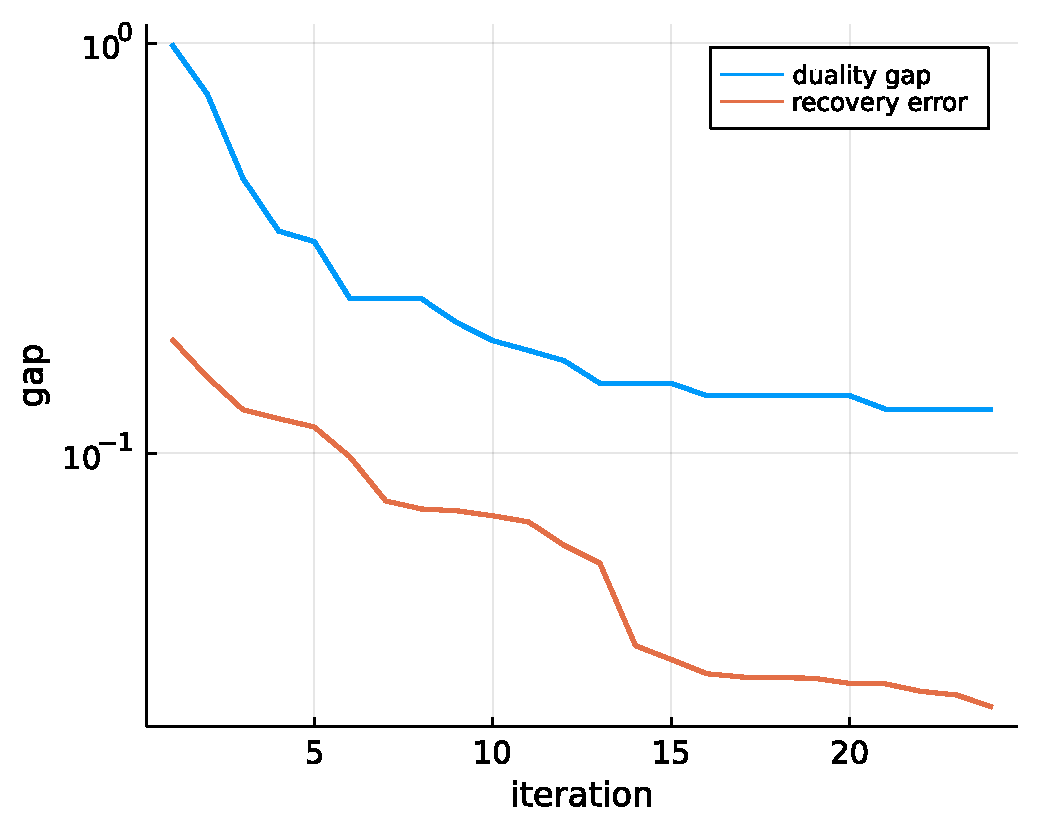
\includegraphics[width=.5\textwidth]{./figures/matrix_completion.pdf}
    \captionsetup{justification=centering}
    \caption{Matrix completion experiment.}
    \label{fig:matrix_completion}
\end{figure}

\subsection{Robust Principal Component Analysis} \label{sec:rpca}

\begin{figure}[t] \label{fig:rpca}
    \begin{subfigure}{.45\textwidth}
      \centering
      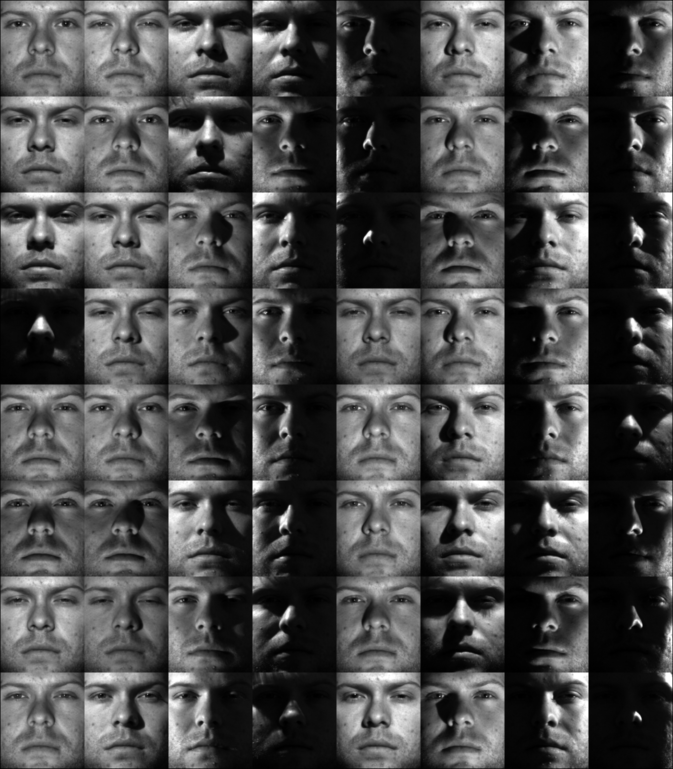
\includegraphics[width=\linewidth]{./figures/face.png}
      \captionsetup{justification=centering}
      \caption{Original faces.}
      \label{fig:face}
    \end{subfigure}
    \hfill
    \begin{subfigure}{.45\textwidth}
      \centering
      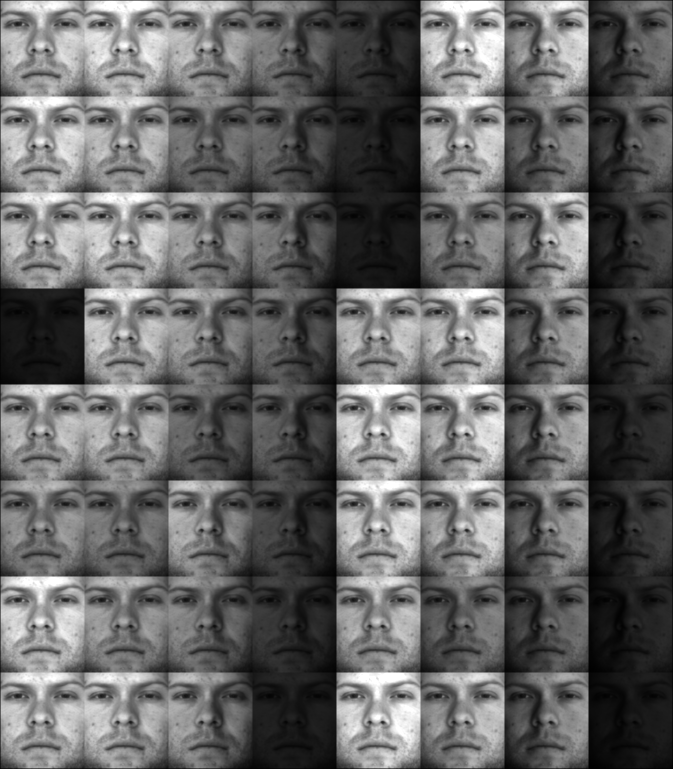
\includegraphics[width=\linewidth]{./figures/faceDeshadow.png}
      \captionsetup{justification=centering}
      \caption{Shadow-removed faces.}
      \label{fig:face_shadow}
    \end{subfigure}
    \captionsetup{justification=centering}
    \caption{Robust principal component analysis experiment.}
\end{figure}

In this section, we show that our primal-retrieval strategy can be applied to more complicated atomic sets besides polyhedral and spectral. We conduct the the similar experiment as in \cite{candes2011robust}. Face recognition algorithms are sensitive to shadows on faces. In order to obtain the best possible performance for these algorithms, it is desired to remove illumination variations and shadows on the face images. We obtained face images from the Yale B face database~\cite{georghiades2001few}. We show the original faces in \autoref{fig:face}, where each face image was of size $192\times 168$ with 64 different lighting conditions. The images were then reshaped into a matrix $M \in \Re^{32256 \times 64}$. Because of the similarity between faces and the sparse structure of the shadow, the matrix $M$ can be approximately decomposed into two components, i.e., 
\[M \approx L + S,\]
where $L$ is a low-rank matrix corresponding to the clean faces and $S$ is sparse matrix corresponding to the shadows. Based on the work by Fan et al.~\cite{fan2020polar}, we know that such decomposition can be obtained via solving the following convex optimization problem:
\begin{equation} \label{eq:rpca}
    \min_{L, S} \enspace \max\{\|L\|_*, \lambda \|S\|_1\}  \enspace \st  \enspace  \|L + S - M\| \leq \alpha.
\end{equation}
By \cite[Proposition~7.3]{fan2019alignment}, we know that \eqref{eq:rpca} is equivalent to 
\begin{equation} \label{eq:rpca2}
    \min_{x} \enspace \gauge\As(x)  \enspace \st  \enspace  \|x - M\| \leq \alpha,
\end{equation}
where $\Ascr = \lambda \Ascr_1 + \Ascr_2$, $\Ascr_1 = \{uv^T \mid u \in \mR^m,\ v \in \mR^n,\ \|u\|_2=\|v\|_2 = 1\}$ and $\Ascr_2 = \{\pm e_ie_j^T \mid i \in [m], j \in [n]\}$. The recovered low-rank component is shown in \autoref{fig:face_shadow}. As we can see from the figure, most of the shadow are successfully removed. This experiment suggests that our primal-retrieval technique can potentially be used for more complex atomic set and allow the underlying the dual-algorithm to produce satisfactory result within a reasonable number of iterations. 

\section{Conclusion}
In this work, we proposed a simple primal-retrieval strategy for atomic-sparse optimization. We demonstrate both theoretically and empirically that our proposed strategy can obtain desirable primal variable given a dual-based algorithm converging to the optimum dual solution. 

Further research opportunities remain, particularly for designing meaningful primal-retrieval strategy for non-polyhedral and non-spectral atomic sets. The primal-retrieval technique developed in this work is algorithm-agnostic, it is possible to develop more efficient primal-retrieval rule that associated with specific optimization algorithms such as the conditional-gradient method.


\section{Proofs}

\subsection{Derivation of duals}\label{app:duals}

We derive the dual problems~\eqref{prob:dual1},~\eqref{prob:dual2} and~\eqref{prob:dual3} using the Fenchel\textendash Rockafellar duality framework. We use the following result.
\begin{theorem}[\protect{\cite[Corollary~31.2.1]{rockafellar1970convex}}]\label{thm-fenchel}
  Let $f_1:\Re^n\to\Re$ and $f_2:\Re^m\to\Re$ be two closed proper convex functions and let $M$ be a linear operator from $\Re^n$ to $\Re^m$, then
  \[\inf_{x \in \Re^n} f_1(x) + f_2(Mx) = \inf_{y \in \Re^m} f_1^*(M^*y) + f_2^*(-y).\]
  If there exist $x$ in the interior of $\dom f_1$ such that $Mx$ in the interior of $\dom f_2$, then strong duality holds, namely both infima are attained. 
\end{theorem}
We also need a result that describes the relationship between gauge, support, and indicator functions. 
\begin{proposition}[\protect{\cite[Proposition~3.2]{fan2019alignment}}] \label{prop-conjugate-gauge}
  Let $C\subset\Re^n$ be a closed convex set that contains the origin. Then 
  \[\gauge_C = \sigma_{C^\circ}=\delta_{C^\circ}^*.\]
\end{proposition}

For problem~\eqref{prob:primal1}, let
\[
  f_1 := \lambda\gauge\As \enspace\text{and}\enspace f_2 := f(b - \cdot)
\]
By the properties of conjugate functions and~\autoref{prop-conjugate-gauge}, we obtain 
\[
  f_1^* =  \delta_{(\frac{1}{\lambda}\Ascr)^\circ} = \delta_{\{x\mid \sigma\As(x)\leq\lambda\}} \enspace\text{and}\enspace f_2^* = \ip{b}{\cdot} + f^*(-\cdot).
\]
Then by~\autoref{thm-fenchel}, we can get the dual problem for~\eqref{prob:primal1} as
\[\minimize{y\in\Re^m} f^*(y) - \ip{b}{y} \enspace\text{subject to}\enspace \sigma\As(M^*y)\leq\lambda.\]

For~\eqref{prob:primal2},
\[f_1 = \delta_{\gauge\As\leq\tau} = \delta_{\tau\Ascr} \enspace\text{and}\enspace f_2 = f(b - \cdot).
\]
By the properties of conjugate functions and~\autoref{prop-conjugate-gauge}, we obtain 
\[f_1^* = \sigma_{\tau\Ascr} = \tau\sigma\As \enspace\text{and}\enspace f_2^* = \ip{b}{\cdot} + f^*(-\cdot).
\]
Then by~\autoref{thm-fenchel}, it follows that the dual problem for~\eqref{prob:primal2} is 
\[\minimize{y\in\Re^m} f^*(y) - \ip{b}{y} + \tau\sigma\As(M^*y).\]

For~\eqref{prob:primal3},
\[
  f_1 = \gauge\As \enspace\text{and}\enspace f_2 = \delta_{\{x\mid f(b - x)\leq\alpha\}}.
\]
By the properties of conjugate functions and~\autoref{prop-conjugate-gauge}, we can get that 
\[
  f_1^* = \delta_{\{x\mid \sigma\As(x)\leq1\}} \enspace\text{and}\enspace f_2^* = \sigma_{\{f(b - x)\leq\alpha\}}.\]
Then by~\cite[Example~E.2.5.3]{hiriart-urruty01}, we know that the support function of the sublevel set is 
\[f_2^* = \sigma_{\{x\mid f(b - x)\leq\alpha\}} = \min_{\beta > 0} \beta\left(f^*\left(-\frac{\cdot}{\beta}\right) + \alpha\right) + \ip{b}{\cdot}.\]
Finally, by~\autoref{thm-fenchel}, we can get the dual problem for~\eqref{prob:primal3} as
\[\minimize{y\in\Re^m,\ \beta > 0} \beta \left( f^*\left( \frac{y}{\beta} \right) + \alpha \right) - \ip{b}{y} \enspace \text{subject to}\enspace \sigma\As(M^* y) \leq 1.\]


\subsection{Proof of Theorem~\ref{thm:p0}} \label{app:main_proof}

The proof of this Theorem relies on the duality between smoothness and strong convexity.
\begin{lemma}[\protect{\cite[Theorem~6]{kakade2009duality}}] \label{lemma:conjugate}
   If $f$ is $L$-smooth, then $f^*$ is $\frac{1}{L}$-strongly convex.
\end{lemma}

\begin{proof}[Proof of Theorem~\ref{thm:p0}]
    \begin{itemize}
      \item[a)] Let $y^*$ denote the optimal dual variable for~\eqref{prob:dual1}. First, we show that $\|y - y^*\|$ can be bounded by the duality gap. Let $g(y) = f^*(y) - \ip{b}{y}$. By~\autoref{lemma:conjugate}, $f^*$ is $\frac{1}{L}$-strongly convex, and it follows that $g$ is also $\frac{1}{L}$-strongly convex. By the definition of strong convexity, 
      \[\forall s \in \partial g(y^*), \enspace g(y) \geq g(y^*) + \ip{s}{y- y^*} + \frac{1}{2L}\|y - y^*\|^2.
      \]
      Optimality requires that 
      \[\exists s \in \partial g(y^*), \enspace \ip{s}{y- y^*} \geq 0 \quad \forall y \enspace\text{s.t.}\enspace \sigma\As(M^*y)\leq\lambda.\]
      Therefore, by reordering the inequality,
      \begin{align}
         \|y - y^*\| & \leq \sqrt{2L(g(y) - g(y^*))}
         \quad \forall x \in \Re^n.
      \end{align} 
    
      Next, we show that $\Escr\As(M^*y^*) \subseteq \Escr\As(M^*y, \epsilon_1)$. For any $a \in \Escr\As(M^*y^*)$, 
      \begin{align*}
        \ip{a}{M^*y} &= \sigma\As(M^*y^*) + \ip{Ma}{y - y^*}
        \\&\geq \sigma\As(M^*y^*) - \left(\max\limits_{a \in \Ascr}\|Ma\|\right)\|y - y^*\|
        \\&\geq \sigma\As(M^*y^*) - \left(\max\limits_{a \in \Ascr}\|Ma\|\right)\sqrt{2L(g(y) - g(y^*))}
        \\&\geq \sigma\As(M^*y) - \epsilon_1,
      \end{align*}
      where the last inequality follows from the fact that $\sigma\As(M^*y^*) = \lambda$ and $y$ is feasible for \eqref{prob:dual3}. 
    
      \item[b)] Let $y^*$ denote the optimal dual variable for~\eqref{prob:dual2}. First, we show that $\|y - y^*\|$ can be bounded by the duality gap. Let $g(y) = f^*(y) - \ip{b}{y} + \tau\sigma\As(M^*y)$. By~\autoref{lemma:conjugate}, $f^*$ is $\frac{1}{L}$-strongly convex, and it follows that $g$ is also $\frac{1}{L}$-strongly convex. 
      By the definition of strongly convex, 
      \[\forall s \in \partial g(y^*), \enspace g(y) \geq g(y^*) + \ip{s}{y- y^*} + \frac{1}{2L}\|y - y^*\|^2.\]
      By optimality, $0 \in \partial g(y^*)$. Reorder the inequality to deduce that
      \[\|y - y^*\|_2 \leq \sqrt{2L(g(y) - g(y^*))}.\]
    
      Next, we show that $\Escr\As(M^*y^*) \subseteq \Escr\As(M^*y, \epsilon_2)$. For any $a \in \Escr\As(M^*y^*)$, 
      \begin{align*}
        \ip{a}{M^*y} &\geq \sigma\As(M^*y^*) - \left(\max\limits_{a \in \Ascr}\|Ma\|\right)\|y - y^*\|
        \\&= \sigma\As(M^*y) - \left(\sigma\As(M^*y) - \sigma\As(M^*y^*)\right) - \left(\max\limits_{a \in \Ascr}\|Ma\|\right)\|y - y^*\|
        \\&\geq \sigma\As(M^*y) - 2\left(\max\limits_{a \in \Ascr}\|Ma\|\right)\|y - y^*\|
        \\&\geq \sigma\As(M^*y) - \epsilon_2.
      \end{align*}
    
      \item[c)] Let $(y^*, \beta^*)$ denote the optimal dual variables for~\eqref{prob:dual3}. First, we show that $\|y - y^*\|$ can be bounded by the duality gap. Let 
      \[g(y) = \beta^*f^* \left(\frac{y}{\beta^*} \right) + \beta^*\alpha - \ip{b}{y}.\] 
      By~\autoref{lemma:conjugate}, $f^*$ is $\frac{1}{L}$-strongly convex, and it's not hard to check that $g$ is $\frac{1}{\beta^*L}$-strongly convex. By the definition of strongly convex,
      \[\forall s \in \partial g(y^*), \enspace g(y) \geq g(y^*) + \ip{s}{y- y^*} + \frac{1}{2\beta^*L}\|y - y^*\|^2.\]
      By optimality,
      \[\exists s \in \partial g(y^*), \enspace\ip{s}{y- y^*} \geq 0 \quad \forall y \enspace\text{s.t.}\enspace \sigma\As(M^*y)\leq1.\]
      Reorder the inequality to deduce that 
      \[\|y - y^*\|_2 \leq \sqrt{2\beta^*L(g(y) - g(y^*))}.\]
    %   \begin{align}
    %      \|y - y^*\|_2 & \leq \sqrt{2\beta^*L(g(y) - g(y^*))} \nonumber \\
    %      & \leq \sqrt{2\beta^*L \left(p_3(x) + d_3(y, \beta^*)\right) } \enspace \forall x \in \Re^n \text{s.t.} f(b - Mx)\leq\alpha\nonumber
    %      \\&\leq \sqrt{2\overline{\beta}L \left(p_3(x) + d_3(y, \beta^*)\right) } \enspace \forall x \in \Re^n \text{s.t.} f(b - Mx)\leq\alpha.
    %   \end{align} 
    
      Since $\beta^*$ is unknown to us, we will then get an upper bound for $d_3(y, \beta^*)$. Fix $y$, let $h(\beta) = d_3(y, \beta)$. By the property of perspective function, we know that $h$ is convex. Then it follows that 
      \[d_3(y, \beta^*) \leq \max\{d_3(y, \underline{\beta}), d_3(y, \overline{\beta})\}.\]
      Therefore,
      \[ \|y - y^*\|_2 \leq \sqrt{2\overline{\beta}L \left( \max\{d_3(y, \underline{\beta}), d_3(y, \overline{\beta})\} - d_3(y^*)\right) } .\]
    
      Finally, we show that $\Escr\As(M^*y^*) \subseteq \Escr\As(M^*y, \epsilon_3)$. For any $a \in \Escr\As(M^*y^*)$, 
      \begin{align*}
        \ip{a}{M^*y} &\geq \sigma\As(M^*y^*) - \left(\max\limits_{a \in \Ascr}\|Ma\|\right)\|y - y^*\|
        \\&= \sigma\As(M^*y) - \left(\sigma\As(M^*y) - \sigma\As(M^*y^*)\right) - \left(\max\limits_{a \in \Ascr}\|Ma\|\right)\|y - y^*\|
        \\&\geq \sigma\As(M^*y) - 2\left(\max\limits_{a \in \Ascr}\|Ma\|\right)\|y - y^*\|
        \\&\geq \sigma\As(M^*y) - \epsilon_3.
      \end{align*}
    \end{itemize}
\end{proof}


\subsection{Upper and lower bounds for \texorpdfstring{$\beta^*$}{} }
\label{app:bounds}
First, we consider~\eqref{prob:dual3}. Let $w = y/\beta$, then~\eqref{prob:dual3} can be equivalently expressed as 
\[\minimize{w} \inf_{\beta>0} \beta(f^*(w) - \ip{b}{w} + \alpha) \enspace\text{subject to}\enspace \sigma\As(M^* w) \leq \beta.\]
Fix $\beta = \beta^*$, then~\eqref{prob:dual3} can be expressed as 
\begin{equation} \label{prob:dual3equiv}
  \minimize{w} f^*(w) - \ip{b}{w} \enspace\text{subject to}\enspace \sigma\As(M^* w) \leq \beta^*.
\end{equation}
Now compare~\eqref{prob:dual3equiv} with~\eqref{prob:dual1} to conclude that they are equivalent when $\lambda = \beta^*$. It thus follows that~\eqref{prob:primal3} is equivalent to  
\begin{equation} \label{prob:p1beta}
    \minimize{x} f(b - Mx) + \beta^*\gauge\As(x). 
\end{equation}   

Next, consider using the level-set method~\cite{aravkin2016levelset} with bisection to solve~\eqref{prob:primal3}. There exists $\tau^* > 0$ such that~\eqref{prob:primal3} is equivalent to
\begin{equation} \label{prob:p2tau}
    \minimize{x} f(b - Mx) \enspace\text{subject to}\enspace \gauge\As(x)\leq\tau^*. 
\end{equation}
With the level-set method, we are able to get $(x_1, \tau_1)$ and $(x_2, \tau_2)$ such that $\tau_1 \leq \tau^* \leq \tau_2$ and $x_i$ is the optimum for 
\begin{equation} \label{prob:p2taui}
    \minimize{x} f(b - Mx) \enspace\text{subject to}\enspace \gauge\As(x)\leq\tau_i, 
\end{equation}
for $i = 1, 2$. Then there exits $\beta_1$ and $\beta_2$ such that $\beta_1 \geq \beta^* \geq \beta_2$ and $x_i$ is optimal for 
\begin{equation} \label{prob:p1betai}
    \minimize{x} f(b - Mx) + \beta_i\gauge\As(x),
\end{equation}
for $i = 1, 2$.

Finally, by~\cite[Theorem~5.1]{fan2019alignment} we can conclude that 
\[\beta_i = \sigma\As(M^*\nabla f(b - Mx_i)) \text{for} i = 1,2.\]
Therefore, we can get upper and lower bounds for $\beta^*$ via level-set method with bisection. Moreover, by strong duality and convergence of the bisection method, the gap between $\beta_1$ and $\beta_2$ will converge to zero. 

\subsection{Proof of Proposition~\ref{prop:polyhedral}}
\label{app:prop_proof}
\begin{proof}
  First, we show that for any $y_i$ such that $\| y_i - y_i^* \| \leq \frac{\delta}{4\| M \|_\Ascr}$, the condition 
  \[\Face\As( M^* y_i^*) \subseteq \texttt{EssCone}(\Ascr, M, y_i, k)\]
  holds. By \autoref{ass:blanket} and the definition of $\delta$-nondegeneracy, we know that 
  \begin{align}
      |  \Face\As( M^* y_i^*) | = k, \quad \text{and} \quad \langle Ma, y_i^* \rangle \leq \sigma_{\Ascr}( M^* y_i^* ) - \delta \quad \forall a \notin \Face\As( M^* y_i^*). \label{eq:Aprime}
  \end{align}
  For any $a \in \Face\As( M^* y_i^*)$, we have
  \begin{align*}
      & \langle a, M^* y_i \rangle \\
      \geq~& \langle a, M^* y_i^* \rangle - | \langle M a, y_i^* - y_i \rangle | \\
      \geq~& \sigma_{\Ascr}( M^* y_i^* ) - \| M \|_\Ascr \frac{\delta}{4\|M\|_{\Ascr}} \\
      \geq~& \sigma_{\Ascr}( M^* y_i^* ) - \frac{\delta}{4}.
  \end{align*}
  For any $a' \notin \Face\As( M^* y_i^*)$, we have 
  \begin{align*}
      & \langle a', M^* y_i \rangle \\
      \leq~ & \langle a', M^* y_i^* \rangle + | \langle M a', y_i^* - y_i \rangle | \\
      \leq~ & \langle a', M^* y_i^* \rangle + \frac{\delta}{4} \\
      \leq~ & \sigma_{\Ascr}( M^* y_i^* ) - \delta + \frac{\delta}{4} \quad \text{(By \autoref{eq:Aprime})} \\
      =~& \sigma_{\Ascr}( M^* y_i^* ) - \frac{3\delta}{4}.
  \end{align*}
    Therefore, 
    \begin{align*}
        \langle a, M^* y_i \rangle > \langle a', M^* y_i \rangle  \quad \forall a \in \Face\As( M^* y_i^*) \text{and} a' \notin \Face\As( M^* y_i^*).
    \end{align*}
    Notice that $\texttt{EssCone}(\Ascr, M, y_i, k)$ contains only the atoms that corresponds to the $k$ largest $\langle a, M^* y_i \rangle$. Therefore $\Face\As( M^* y_i^*) \subseteq \texttt{EssCone}(\Ascr, M, y_i, k)$.
    
    By the assumption $y_i^{(t)} \to y_i^*$. For $i \in \{1,2,3\}$, we know there exist $T_i > 0$ such that $\| y_i^{(t)} - y_i^* \| < \frac{\delta}{4\| M \|_\Ascr}$ for all $t > T$. Therefore $\Face\As( M^* y_i^*) \subseteq \texttt{EssCone}(\Ascr, M, y_i^{(t)}, k)~~\forall t > T$ and we complete the proof.
\end{proof}

\subsection{Proof for \autoref{thm:svd_approx_score}}
\begin{proof}
  By the definition of $\rho(\cdot, \cdot)$, it follows that
  \[
    \rho(A, C) \leq \rho(B, C) \quad \forall A, B, C \subseteq \mR^{n \times m} ~\text{such that}~ A \subseteq B.
  \]
  We know that $ \Face\As( M^* y^* ) \subseteq  \Face\As( M^* y, \epsilon )$, then obviously we have 
  \[
    \rho( \Face\As( M^* y^* ), \widehat{\Ascr}  ) \leq \rho( \Face\As( M^* y, \epsilon ), \widehat{\Ascr}  ).
  \]
  For any $\Ascr_1, \Ascr_2 \subseteq \Ascr$,
  \begin{align}
    \rho( \Ascr_1, \Ascr_2 ) = \sqrt{ \adjustlimits\sup_{a_1 \in \Ascr_1} \inf_{a_2 \in \Ascr_2} \| a_1 - a_2 \|_F^2 } = \sqrt{ 2 - 2 \left( \adjustlimits \inf_{a_1 \in \Ascr_1} \sup_{a_2 \in \Ascr_2} \ip{a_1}{a_2} \right) }, \label{eq:norm2ip}
  \end{align}
  where the second equality holds since $\| a_1 \|_F = \| a_2 \|_F = 1$ by the definition of $\Ascr$. Define $\Ascr_1 = \Face\As( M^* y, \epsilon )$ and $\Ascr_2 = \widehat{\Ascr} = \{ U_r p q^T V_r^T | \|p\|_2 = \|q\|_2 = 1 \}$, where $U_r, V_r$ are the top-$r$ singular vectors of $M^*y$. Let $k \coloneqq \min\{n,m\}$, $\Cscr_1 = \{(p, q) \mid \sum_{i=1}^{k} \sigma_i p_i q_i \geq \sigma_1 - \epsilon,~ \|p\|_2 = \|q\|_2 = 1, ~p,q \in \mR^{ k }\}$ and $\Cscr_2 = \{(\hat{p}, \hat{q}) \mid \|\hat{p}\|_2 = \|\hat{q}\|_2 = 1, ~\hat{p},\hat{q} \in \mR^{ k }\}$, then
  \begin{align}
    \rho( \Ascr_1, \Ascr_2  ) & = \sqrt{ 2 - 2 \left( \min_{p, q \in \Cscr_1} \max_{ \hat{p}, \hat{q} \in \Cscr_2} \ip{ Up q^T V^T }{ U_r \hat{p} \hat{q}^T V_r^T } \right) } \nonumber \\
    & = \sqrt{ 2 - 2 \left( \min_{p, q \in \Cscr_1} \max_{ \hat{p}, \hat{q} \in \Cscr_2} \left( \sum_{i=1}^r p_i \hat{p}_i \right) \left( \sum_{i=1}^r q_i \hat{q}_i \right) \right) } \nonumber \\
    & = \sqrt{ 2 - 2 \left(\min_{p, q \in \Cscr_1} \| p_{1:r} \|_2 \| q_{1:r} \|_2 \right) } \label{eq:rho_exp} 
    % \text{subject to} & \sum_{i=1}^{k} \sigma_i p_i q_i \geq \sigma_1 - \epsilon,~ \|p\|_2 = \|q\|_2 = 1, ~p,q \in \mR^{ k }, \nonumber \\
  \end{align}
  Now we consider the subproblem in \eqref{eq:rho_exp}: 
  \begin{align}
    \min_{p,q}\enspace & \| p_{1:r} \|_2 \| q_{1:r} \|_2 \label{eq:reduced_p1} \tag{P$_1$} \\
    \text{subject to} & \sum_{i=1}^{k} \sigma_i p_i q_i \geq \sigma_1 - \epsilon,~ \|p\|_2 = \|q\|_2 = 1, ~p,q \in \mR^{ k }. \nonumber
  \end{align}
  If $p^*$ and $q^*$ is a solution of the problem \eqref{eq:reduced_p1}, then it's easy to verify that 
  \begin{align*}
    & \tilde{p} = \left[ \| p^*_{1:r} \|_2, 0,\ldots, \|p^*_{r+1:k}\|_2, 0, \ldots, 0 \right] \\ 
    \text{and} ~& \tilde{q} = \left[ \| q^*_{1:r} \|_2, 0,\ldots, \|q^*_{r+1:k}\|_2, 0, \ldots, 0 \right]
  \end{align*}
  is also a valid solution. Therefore there must exist solution $p^*, q^*$ such that $p_i = q_i = 0~\forall i \notin \{1, r+1\}$, that is only $p^*_1, q^*_1$ and $p^*_{r+1}$ and $q^*_{r+1}$ are greater or equal than 0. This allow us to further reduce the problem to
  \begin{align*}
    \min_{ p_1, q_1, p_{r+1}, q_{r+1} } &~  p_1 q_1 \\
    \text{subject to} & \sigma_1 p_1 q_1 + \sigma_{r+1} p_{r+1} q_{r+1} \geq \sigma_1 - \epsilon, \\
    & p_1^2 + p_{r+1}^2 = q_1^2 + q_{r+1}^2 = 1, ~p_1, q_1, p_{r+1}, q_{r+1} \geq 0. 
  \end{align*}
  It's easy to verify that when $\sigma_1 - \sigma_{r+1} \geq \epsilon$, the above problem attains solution at 
  \[
    p_1 = q_1 = \sqrt{\frac{\sigma_1 - \sigma_{r+1} - \epsilon}{ \sigma_1 - \sigma_{r+1} } } \text{and} p_{r+1} = q_{r+1} = \sqrt{1 - p_1^2}.
  \]
  When $\sigma_1 - \sigma_{r+1} < \epsilon$, the solution is simply $p_1 = q_1 = 0, p_{r+1}= q_{r+1} = 1$.
  Therefore the optimal value of \eqref{eq:reduced_p1} is $\max\{1 - \epsilon / ( \sigma_1 - \sigma_{r+1} ), 0\}$, plug this into \autoref{eq:rho_exp} and the proof is finished. 
\end{proof}

\begin{proposition}[Hausdorff error bound] \label{prop:dist_to_sol}
    Given $\widehat{\Ascr} \subseteq \Ascr$ such that , there exists $ x \in \cone ( \widehat{\Ascr} ) $ such that 
    \begin{equation}
            \| x - x^* \|_F \leq \dist( \suppa(x^*), \widehat{\Ascr} )\cdot \sqrt{| \suppa(x^*) |} \cdot \| x^* \|_F.  \label{eq:dist_to_sol}
    \end{equation}
\end{proposition}

\subsection{Proof of \autoref{prop:spectral}}
\begin{proof}
  By \autoref{prop:dist_to_sol}, we know that there exist $\tilde{x}$ satisfies \autoref{eq:dist_to_sol}.
  Then by the $L$-smoothness of $f$,
  \begin{align}
      f( b - M \tilde{x} ) &~\leq~ f( b - M x^* ) + \langle \nabla f( b - M x^* ), M( x^* - \tilde{x} ) \rangle + \frac{L}{2} \| M( x^* - \tilde{x} ) \|^2  \nonumber \\
      &~\leq~ f( b - M x^* ) + \| \nabla f( b - M x^* ) \| \| M( x^* - \tilde{x} ) \| + \frac{L}{2} \| M( x^* - \tilde{x} ) \|^2. \label{eq:errorBoundIntermediate1}
  \end{align}
  By the smoothness and convexity of $f$, we further have
  \begin{align*}
      \| \nabla f( b - M x^* ) - \nabla f(0) \|^2 \leq 2L ( f(b - M x^*) - f(0) ).
  \end{align*}
  Note that $f(0)$ and $\nabla f(0) = 0$, the above reduces to $\| \nabla f( b - M x^* ) \| \leq \sqrt{2 L \alpha}$. Combining with \autoref{eq:errorBoundIntermediate1}, we obtain
  \begin{align*}
      f( b - M \tilde{x} ) &~\leq~ f( b - M x^* ) + \sqrt{2 L \alpha} \| M( x^* - \tilde{x} ) \| + \frac{L}{2} \| M( x^* - \tilde{x} ) \|^2 \\
      &~\leq~ f( b - M x^* ) + \sqrt{2 L \alpha} \| M \| \rho( \suppa(x^*), \widehat{\Ascr} )\cdot \sqrt{| \suppa(x^*) |} \cdot \| x^* \|_F  \\
      &\qquad + \frac{L}{2} \rho( \suppa(x^*), \widehat{\Ascr} )^2 | \suppa(x^*) | \| x^* \|_F^2.
  \end{align*}
\end{proof}
























